\chapter{Results}
\label{chapter:results}

We obtain results for our two sub-tasks on selected popular datasets. The results are reported using standard metrics commonly used to evaluate these tasks. 


\section{Multi Object Tracking Evaluation}

\subsection{Datasets and Evaluation metrics}
Experiments are conducted on the MOT16 \cite{DeepSiam:MilanL0RS16} and KITTI \cite{DeepSiam:KITTI} tracking datasets. The MOT16 dataset contains 7 videos in its training set. The KITTI tracking dataset contains 21 videos in its training set. The Siamese Network for appearance consistency is trained completely on external data (ImageNet datasets) and there is no overlap with any of the MOT16 or KITTI data. The LSTM network is trained only with the use of bounding box locations of objects and class information for a partition of the training sets of these two datasets (the remainder is kept aside for testing purposes). Results are reported for our test partition (in the case of LSTM usage) and for the entire datasets (in cases they are not used for training).
\par Evaluation of our system is carried out for the entire system as well as for the study of LSTM network alone. For the case of the entire system, we consider the metrics used by the MOT benchmarks for evaluation. This includes Multiple Object Tracking Accuracy (MOTA), Multiple Object Tracking Precision (MOTP), the ratio of Mostly Tracked targets (MT), and the ratio of Mostly Lost targets (ML). In the case of the LSTM network, the Average Precision (AP) value for the predicted frames across the dataset and classes is reported.

\subsection{Evaluation}
The evaluations on the MOT16 Dataset for the end to end system are reported in Table I. Evaluations mainly focus on two aspects: improvement in accuracy with the introduction of the similarity measure to a traditional tracker using only a Kalman filter or an LSTM network and how closely related the accuracy is with state of the art multi-object trackers. Similar results on the KITTI tracking dataset are presented for our work alongside comparisons (note that few state-of-the-art works report on this dataset) in Table II. Separate evaluations for the LSTM in the case of single object tracking for individual tracklets in the KITTI dataset was carried out. An average IoU of 61.45 and AP of 0.96 at 0.5 IoU were obtained for this experiment.

\begin{table*}[ht]
	\caption[Results on MOT Dataset]{Comparison  of  our  performance  on  MOT16  dataset  with  recent  works}
	\label{MOT16 Results}
	\begin{center}
		\begin{tabular}{|c||c||c||c||c||c|}
			\hline
			Method & Mode & MOTA$\uparrow$ & MOTP$\uparrow$ & MT$\uparrow$ & ML$\downarrow$\\
			\hline
			Deep SORT \cite{DeepSiam:deepSort} & ONLINE & 61.40\% & 79.10\% & 32.80\% & 18.20\%\\
			\hline
			SORT \cite{DeepSiam:Sort} & ONLINE & 59.80\% & 79.60\% & 25.40\% & 22.70\%\\
			\hline
			RNN LSTM \cite{DeepSiam:multitarget} & ONLINE & 19.00\% & 71.00\% & 05.50\% & 45.60\%\\
			\hline
			MDP \cite{DeepSiam:learntotrack} & ONLINE & 30.30\% & 71.30\% & 13.00\% & 38.40\%\\
			\hline
			DMAN \cite{DeepSiam:attention} & ONLINE & 46.10\% & 73.80\% & 17.40\% & 42.70\%\\
			\hline
			LSTM+Similarity (Ours) & ONLINE & 66.70\% & 69.00\% & 39.18\% & 16.80\%\\
			\hline
			Kalman Filter (Ours) & ONLINE & 61.00\% & 69.00\% & 17.00\% & 17.00\%\\
			\hline
		\end{tabular}
	\end{center}
\end{table*}

\begin{table*}[h]
	\caption[Results on KITTI dataset]{Comparison  of  our  performance  on  KITTI-trracking  dataset  with  recent  works}
	\label{KITTI Results}
	\begin{center}
		\begin{tabular}{|c||c||c||c||c||c|}
			\hline
			Method & Mode & MOTA$\uparrow$ & MOTP$\uparrow$ & MT$\uparrow$ & ML$\downarrow$\\
			\hline
			Regionlets Only \cite{DeepSiam:kalman} & ONLINE & 76.40\% & 81.50\% & 54.10\% & 9.30\%\\
			\hline
			MS-CNN Only \cite{DeepSiam:kalman} & ONLINE & 81.23\% & 85.60\% & 66.30\% & 4.60\%\\
			\hline
			Regionlets MS-CNN \cite{DeepSiam:kalman} & ONLINE & 82.60\% & 85.00\% & 70.50\% & 5.30\%\\
			\hline
			SMES \cite{DeepSiam:simmap} & ONLINE & 70.78\% & 80.38\% & 51.68\% & 7.77\%\\
			\hline
			LSTM + Similarity (Ours) & ONLINE & 83.58\% & 78.50\% & 48.23\% & 2.25\%\\
			\hline
		\end{tabular}
	\end{center}
\end{table*}


\subsection{Experiments to analyze the extensibility of the modules}

LSTM based data association for end to end trainability: The LSTM network was trained under negative log likelihood loss. It was observed that network was not developing a significant convergence even for a fixed set of data associations which was also the key expectation. This methodology is trainable but in comparison to the results from the Hungarian algorithm, the associations are sub-optimal and have a significant potential of resulting in non-coherent results (similar to observations at the training phase) which deprecate the accuracy of the entire system henceforth. The results being inconsistent as well as non-coherent and the observation that training sessions do not converge to a feasible setting made this sub module unsuccessful in terms of performance.

Feature Predictor: The feature space is significant in every novel approach considered in the fields of vision based analysis where tracking is only a sub group of it. Along with the ability of the LSTM networks to perform well in prediction, and as model predictors used in current trackers perform linear interpolation of the feature tensors, an experiment on the ability of a trainable network to predict the feature space was conducted (generic interpolation of features is done in most of the Siamese tracking networks and they are proven to perform well in practice).
During this analysis, a robust LSTM network with high hidden state size was trained on the extracted features in sequences. (Ability to compare a complete feature vector can be integrated for optical flow analysis and many further approaches if turns out to be successful). However the feature predicting network was over fitting to the dataset (custom) during the training phase. The accuracy of the tests for network validation was poor and turned out insufficient for any further analysis.


\section{Panoptic Segmentation Evaluation}

In this section, we first show the convergence of the mean field based inference algorithm for BCRF and then show the usefulness of the BCRF model by evaluating its performance on the Pascal VOC dataset and the COCO dataset.

\subsection{Convergence of the Inference}
\begin{figure}[t]
\vspace{-0.7cm}
  \centering
  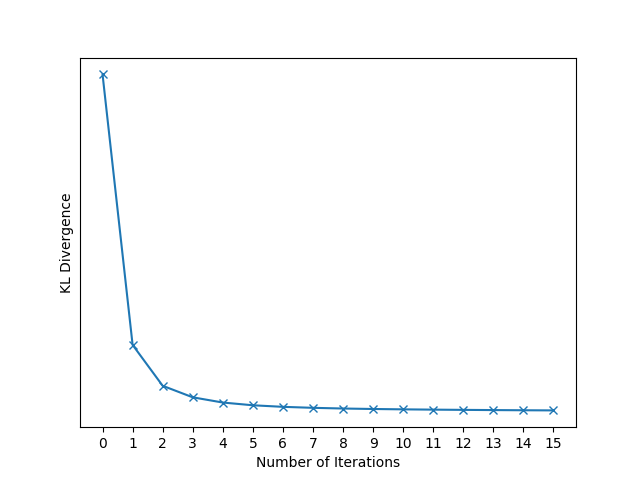
\includegraphics[ width=0.5\textwidth]{figs/kl_div.png}
  \vspace{-0.3cm}
  \caption[Convergence of BCRF Inference]{{\bf Convergence of BCRF Inference.} Convergence of KL divergence with the number of iterations.\vspace{0.0cm}}
  \label{fig:kl_div}
\vspace{0.5cm}
\end{figure}

It is difficult to provide a theoretical convergence guarantee for mean field algorithms with parallel updates~\cite{Higherorder_mf, Koller_book}. We therefore provide empirical evidence to show that the presented mean field inference algorithm for our BCRF with cross potentials converge under normal conditions. To this end, we estimate the KL divergence between the original joint distribution and the factorized distribution (see Eq.~\eqref{eq:q_approx}), at the end of each iteration in Algorithm~\ref{alg:infer}. Note that this KL divergence can be estimated up to a constant using the method described in ~\cite{densecrf_suppl}. We pick 20 random images from the Pascal VOC validation set and average the KL divergence for each iteration across these images. The resulting plot is shown in Fig.~\ref{fig:kl_div}. It can be seen that the KL divergence measure, and therefore the inference algorithm, converges within a few iterations. We also note that visual results do not change after about 5 iterations.

\subsection{Bipartite Potentials Learning}
Figure \ref{fig:potentials} illustrates how important logits belonging to each class in the instance branch are for predicting each class in the semantic branch when the model has been fully trained. Our BCRF module allows the network to learn complex relationships between the semantic and instance features belonging to each class. While there is room for it to learn a simple logical relationship, the variation of learned parameters in Figure \ref{fig:potentials} verifies that a complex class-specific mapping has been learned by the network. 

\subsection{Results on the Pascal VOC Dataset}

In this experiment we use the architecture shown in Figure~\ref{fig:bcrf_net} and CNN components similar to the ones used in~\cite{Upsnet_paper}. More specifically, we use a ResNet-50 with an FPN as the backend, to which we attach a fully convolutional network as the semantic segmentation head and a Mask R-CNN network as the instance segmentation head. 

During both training and inference we used 5 mean-field iterations for BCRF. At the output, we calculate the loss function as a summation of two components: the usual pixel-wise categorical cross entropy loss for the semantic component~\cite{FCN_2015} and the loss used in~\cite{Anurag17} for the instance component. We used full-image training with batch size 1 and SGD with learning rate $0.0007$ and momentum $0.99$. In Table~\ref{tbl:pascal_e2e}, we report the summary of the quantitative results. Table~\ref{tbl:pascal_detailed} shows the class-wise results. Qualitative results are shown in Table~\ref{tbl:pascal_visual}, where benefits of optimally combining the semantic segmentation classification and instance segmentation classification with BCRF can be seen.

\begin{table}[]\centering
	\begin{tabular}{|c|c|c|c|}
		\hline
		\textbf{Method} & \textbf{PQ} & \textbf{SQ} & \textbf{RQ} \\ \hline
		DeeperLab \cite{deeperLab}      & 67.35       & -           & -           \\ \hline
		Ours (baseline) & 70.50       & 88.65       & 78.83       \\ \hline
		Ours (CRF only) & 67.72       & 87.62       & 76.48       \\ \hline
		Ours (BCRF)     & 71.76       & 89.63       & 79.33       \\ \hline
	\end{tabular}
	\vspace{-0.2cm}
	\caption[Comparison of results on Pascal VOC dataset]{Comparison of results on Pascal VOC dataset. The baseline used contains DeepLab-v3 for semantic branch and Mask-RCNN for instance branch followed by combination using the simple logical method outlined in \cite{panoptickirillov2017}. CRF only corresponds to setting the BCRF cross-potential terms to zero. BCRF is our complete network.}
	\label{tbl:pascal_e2e}
	\vspace{0.5cm}
\end{table}
\begin{table*}[t]
	\vspace{-0.2cm}
	\hspace{0.2cm}
	\centering
	{\arraybackslash
\begin{tabular}{l|c|c|c|c|c|c}
	\hline
	\textbf{}	         & \multicolumn{2}{c|}{\textbf{PQ}} & \multicolumn{2}{c|}{\textbf{SQ}} & \multicolumn{2}{c}{\textbf{RQ}}  \\ \hline
	\textbf{Class}       & W/O BCRF       & BCRF            & W/O BCRF        & BCRF           & W/O BCRF        & BCRF           \\ \hline
	\textbf{Background}  & 90.8           & 92.33           & 93.39           & 94.69          & 97.22           & 97.51          \\ \hline
	\textbf{Aeroplane}   & 78.55          & 80.37           & 88.57           & 92.6           & 88.68           & 86.79          \\ \hline
	\textbf{Bicycle}     & 29.78          & 31.71           & 67.36           & 68.46          & 44.21           & 46.32          \\ \hline
	\textbf{Bird}        & 84.98          & 85.09           & 93.05           & 93.24          & 91.32           & 91.25          \\ \hline
	\textbf{Boat}        & 65.83          & 66.21           & 85.33           & 86.48          & 77.14           & 76.56          \\ \hline
	\textbf{Bottle}      & 67.44          & 64.05           & 92.05           & 90.68          & 73.26           & 70.63          \\ \hline
	\textbf{Bus}         & 82.68          & 82.58           & 94.56           & 95.46          & 87.44           & 86.51          \\ \hline
	\textbf{Car}         & 72.22          & 70.93           & 93.69           & 91.7           & 77.08           & 77.35          \\ \hline
	\textbf{Cat}         & 77.41          & 83.4            & 91.24           & 93.73          & 84.85           & 88.97          \\ \hline
	\textbf{Chair}       & 43.3           & 41.79           & 82.5            & 82.64          & 52.49           & 50.57          \\ \hline
	\textbf{Cow}         & 76.91          & 80.42           & 92.81           & 93.95          & 82.87           & 85.6           \\ \hline
	\textbf{Diningtable} & 51.33          & 51.8            & 80.81           & 82.88          & 63.51           & 62.5           \\ \hline
	\textbf{Dog}         & 76.63          & 81.59           & 90.5            & 93.29          & 84.67           & 87.46          \\ \hline
	\textbf{Horse}       & 76.86          & 81.4            & 89.38           & 91.11          & 86              & 89.34          \\ \hline
	\textbf{Motorbike}   & 78.07          & 80.21           & 87.5            & 89.89          & 89.23           & 89.23          \\ \hline
	\textbf{Person}      & 76.33          & 77              & 89.75           & 89.73          & 85.05           & 85.81          \\ \hline
	\textbf{Pottedplant} & 58.98          & 60.62           & 85.41           & 85.32          & 69.06           & 71.05          \\ \hline
	\textbf{Sheep}       & 74.29          & 74              & 93.86           & 93.48          & 79.15           & 79.15          \\ \hline
	\textbf{Sofa}        & 60.37          & 62.12           & 88.47           & 89.5           & 68.24           & 69.41          \\ \hline
	\textbf{Train}       & 78.52          & 80.05           & 88.7            & 90.43          & 88.52           & 88.52          \\ \hline
	\textbf{Tvmonitor}   & 79.23          & 79.34           & 92.8            & 92.93          & 85.38           & 85.38          \\ \hline
	\textbf{Mean Value}  & \textbf{70.5}  & \textbf{71.76}  & \textbf{88.65}  & \textbf{89.63} & \textbf{78.83}  & \textbf{79.33} \\ \hline
\end{tabular}
	}
	\vspace{0.0cm}
	\caption[Detailed results on the Pascal VOC dataset]{\label{tbl:pascal_detailed}{\bf Pascal VOC dataset.} Detailed class-wise panoptic segmentation results on the Pascal VOC validation set comparing results without BCRF vs with BCRF on a standard network.}
	\vspace{0.5cm}
\end{table*}


\begin{table*}[h!]
\vspace{-0.8cm}
%  \centering
	\begin{subtable}{\textwidth}
        \centering
        {\renewcommand{\arraystretch}{0.7}
                                \begin{tabular}{ c@{\hspace{3pt}} c@{\hspace{3pt}} c@{\hspace{3pt}} c@{\hspace{3pt}} c}				
						
\includegraphics[width=0.19\textwidth]{figs/pascal/original/144.jpg}%
						& 
\includegraphics[width=0.19\textwidth]{figs/pascal/before_sem/144.png}%
						& 
\includegraphics[width=0.19\textwidth]{figs/pascal/before_ins/144.png}%
						& 
\includegraphics[width=0.19\textwidth]{figs/pascal/after_sem/144.png}%
						& 
\includegraphics[width=0.19\textwidth]{figs/pascal/after_ins/144.png}\\
														\newline
						\includegraphics[width=0.19\textwidth]{figs/pascal/original/421.jpg}%
						& 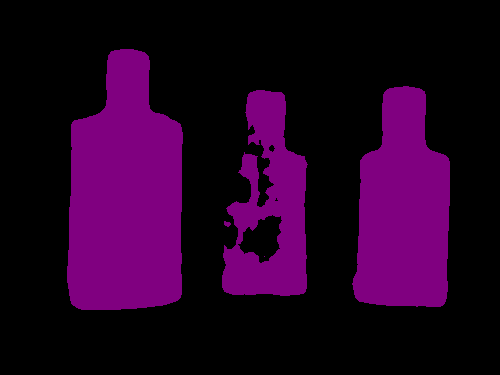
\includegraphics[width=0.19\textwidth]{figs/pascal/before_sem/421.png}%
						& 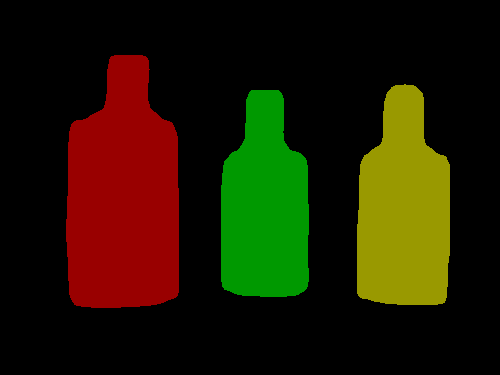
\includegraphics[width=0.19\textwidth]{figs/pascal/before_ins/421.png}%
						& \includegraphics[width=0.19\textwidth]{figs/pascal/after_sem/421.png}%
						& 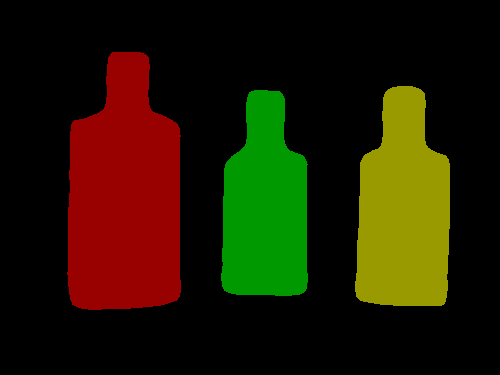
\includegraphics[width=0.19\textwidth]{figs/pascal/after_ins/421.png}\\
						                                \newline
						\includegraphics[width=0.19\textwidth]{figs/pascal/original/438.jpg}%
						& 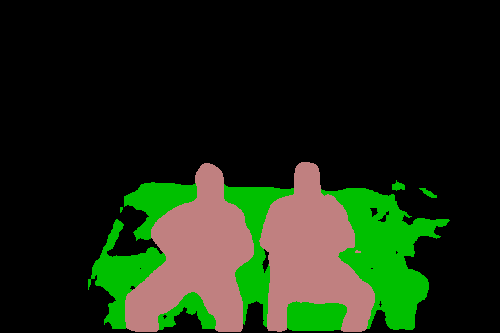
\includegraphics[width=0.19\textwidth]{figs/pascal/before_sem/438.png}%
						& 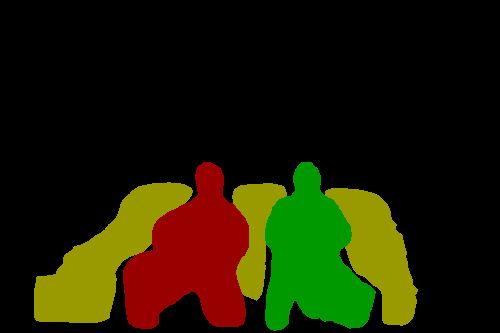
\includegraphics[width=0.19\textwidth]{figs/pascal/before_ins/438.png}%
						& \includegraphics[width=0.19\textwidth]{figs/pascal/after_sem/438.png}%
						& 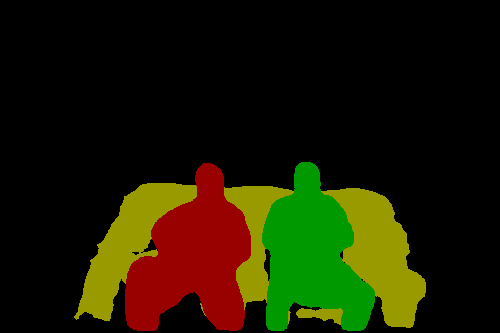
\includegraphics[width=0.19\textwidth]{figs/pascal/after_ins/438.png}\\
						                               \newline
						\includegraphics[width=0.19\textwidth]{figs/pascal/original/468.jpg}%
						& 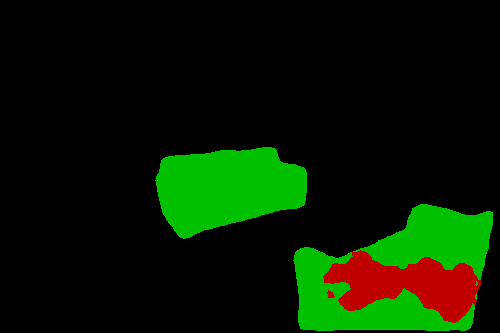
\includegraphics[width=0.19\textwidth]{figs/pascal/before_sem/468.png}%
						& 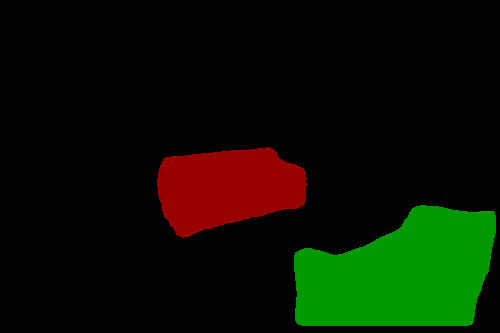
\includegraphics[width=0.19\textwidth]{figs/pascal/before_ins/468.png}%
						& \includegraphics[width=0.19\textwidth]{figs/pascal/after_sem/468.png}%
						& 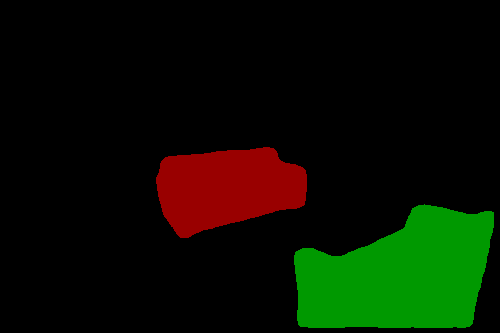
\includegraphics[width=0.19\textwidth]{figs/pascal/after_ins/468.png}\\
														\newline
						\includegraphics[width=0.19\textwidth]{figs/pascal/original/184.jpg}%
                        & 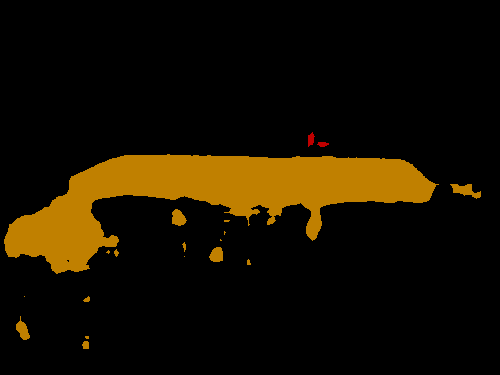
\includegraphics[width=0.19\textwidth]{figs/pascal/before_sem/184.png}%
                        & \includegraphics[width=0.19\textwidth]{figs/pascal/before_ins/184.png}%
                        & 
\includegraphics[width=0.19\textwidth]{figs/pascal/after_sem/184.png}%
                        & 
\includegraphics[width=0.19\textwidth]{figs/pascal/after_ins/184.png}\\
                                                        \newline
						\includegraphics[width=0.19\textwidth]{figs/pascal/original/226.jpg}%
                        & \includegraphics[width=0.19\textwidth]{figs/pascal/before_sem/226.png}%
                        & 
\includegraphics[width=0.19\textwidth]{figs/pascal/before_ins/226.png}%
                        & 
\includegraphics[width=0.19\textwidth]{figs/pascal/after_sem/226.png}%
                        & 
\includegraphics[width=0.19\textwidth]{figs/pascal/after_ins/226.png}\\
%                                                          \newline
%  						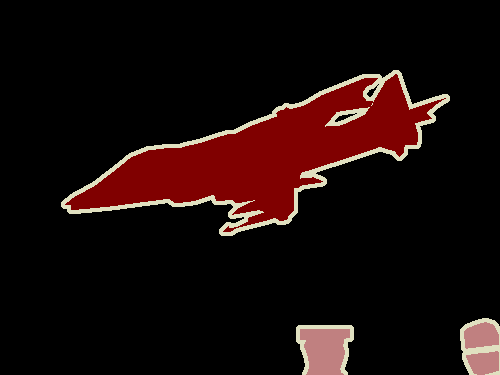
\includegraphics[width=0.19\textwidth]{figs/pascal/original/233.jpg}%
%                          & 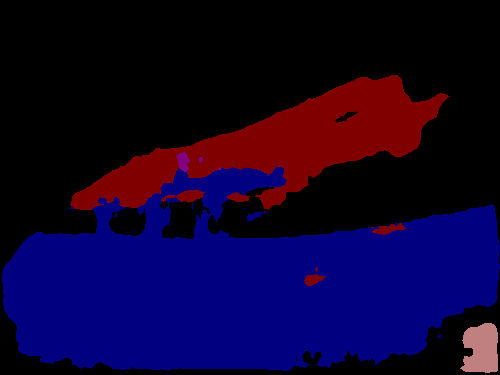
\includegraphics[width=0.19\textwidth]{figs/pascal/before_sem/233.png}%
%                          & 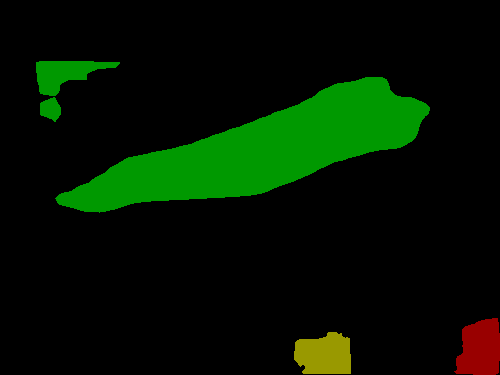
\includegraphics[width=0.19\textwidth]{figs/pascal/before_ins/233.png}%
%                          & 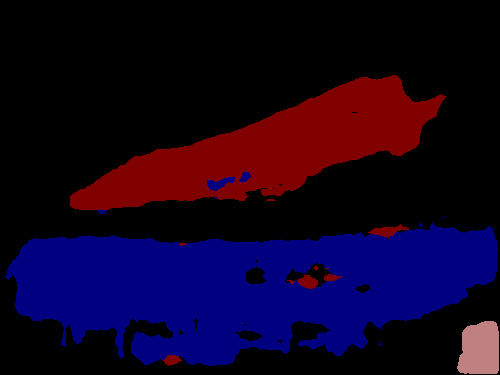
\includegraphics[width=0.19\textwidth]{figs/pascal/after_sem/233.png}%
%                          &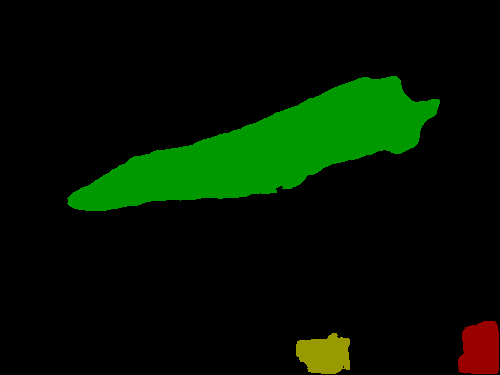
\includegraphics[width=0.19\textwidth]{figs/pascal/after_ins/233.png}\\														
% 														
                                \end{tabular}
                                }
    \end{subtable}
    \vspace{0.0cm}
    \caption[Visualizations on Pascal VOC]{{\bf Visualizations on Pascal VOC.} Example images from the Pascal VOC validation set. Columns left to right: original image, semantic output before BCRF, instance output before BCRF, semantic output after BCRF, instance output after BCRF. Each row contains a new image. The standard Pascal VOC color map is used for the semantic segmentation results.}
    \label{tbl:pascal_visual}
    \vspace{0.1cm}
\end{table*}


\subsection{Results on the COCO Dataset}
To further evaluate the usefulness of BCRF without any efforts for end-to-end training, experiments were conducted on the COCO dataset by simply plugging in the BCRF on an existing pre-trained model. We used a combination of publicly available models of~\cite{Upsnet_paper, object_detection_api}, which produced a PQ score of 41.4\% on the COCO validation set. The parameters of the BCRF were hand-tuned using a small subset of train images. Results obtained from that BCRF model without end-to-end training are listed in Table~\ref{tbl:coco_values}.

\begin{table*}[t]
\vspace{-0.2cm}
\hspace{0.2cm}
\centering
{\arraybackslash
\begin{tabular}{c|c|c|c|c|c|c|c}
	\hline
	& \multicolumn{2}{c|}{\textbf{PQ}} & \multicolumn{2}{c|}{\textbf{SQ}} & \multicolumn{2}{c|}{\textbf{RQ}} &         \\ \hline
	\textbf{Category} & W/O BCRF          & BCRF         & W/O BCRF          & BCRF         & W/O BCRF          & BCRF         & Classes \\ \hline
	\textbf{All}      & 41.4              & 41.7         & 78.3              & 79.1         & 50.8              & 51.1         & 133     \\
	\textbf{Things}   & 47.4              & 47.4         & 80.4              & 80.4         & 57.3              & 57.3         & 80      \\
	\textbf{Stuff}    & 32.5              & 33.2         & 75.1              & 77.1         & 40.9              & 41.6         & 53      \\ \hline
\end{tabular}
}
\vspace{0.0cm}
\caption[Results on COCO dataset]{\label{tbl:coco_values}{\bf COCO dataset.} Panoptic segmentation results on the COCO validation set.}
\vspace{0.5cm}
\end{table*}




\begin{figure}[t]
	\begin{center}
		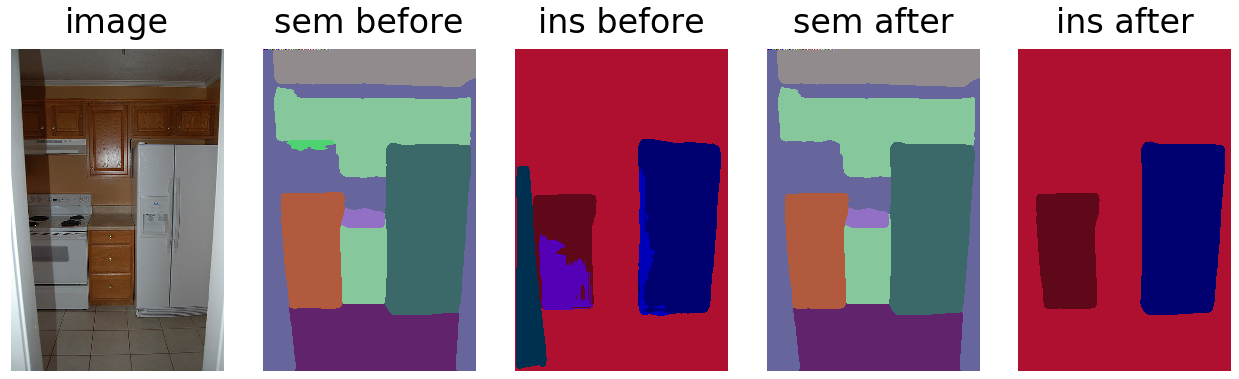
\includegraphics[width=\linewidth]{figs/stuff_vis.png}
	\end{center}
	\vspace{-0.5cm}
	\caption{Visualisation of improvements on COCO Dataset}
	\label{fig:vis}
	\vspace{0.5cm}
\end{figure}

\subsection{BCRF learns beyond simple logical mapping}
Figure \ref{fig:potentials} illustrates how important logits belonging to each class in the instance branch are for predicting each class in the semantic branch when the model has been fully trained. Our BCRF module allows the network to learn complex relationships between the semantic and instance features belonging to each class. While there is room for it to learn a simple logical relationship, the variation of learned parameters in Figure \ref{fig:potentials} verifies that a complex class-specific mapping has been learned by the network. 

\begin{figure}[t]
	\begin{center}
		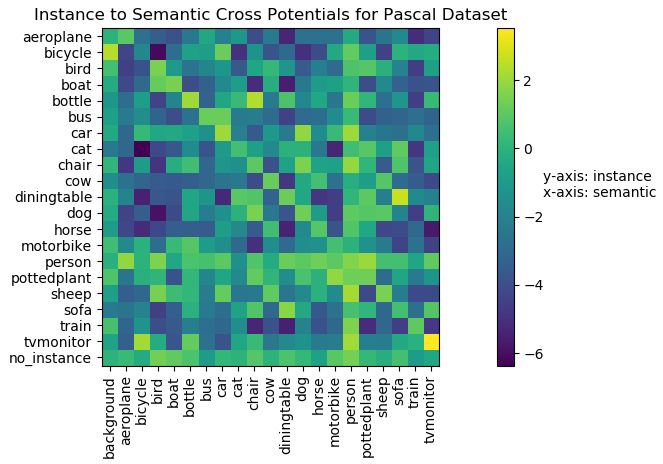
\includegraphics[width=0.8\linewidth]{figs/ins_to_sem.png}
	\end{center}
	\vspace{-0.4cm}
	\caption[Bipartite Potentials Visualization]{The heatmap illustrates inter-class dependencies learned by the cross-potential term weights of BCRF. Note that a logarithmic scale has been used. }
	\label{fig:potentials}
	\vspace{0.5cm}
\end{figure}